\documentclass[11]{article}

\usepackage{amsmath}
\usepackage{fontenc}
\usepackage{graphicx}
\usepackage{stfloats}
\usepackage{fullpage}

% In case you need to adjust margins:
%\topmargin=-0.45in      %
%\evensidemargin=0in     %
%\oddsidemargin= 0in      %
%\textwidth=6.5in        %
%\textheight=9.0in       %
%\headsep=0.25in         %

\author{Marissa Hollingsworth}
\title{Performance and Usability of FUSE-DFS: A Filesystem in Userspace Module for the Hadoop Distributed File System} 

\begin{document}
\maketitle

\section{Introduction}
Distributed filesystems allow multiple users on multiple machines to 
access files and storage resources from multiple hosts who share 
resources through a network. Distributed filesystems strive to maintain
high performance while providing transparent replication and fault 
tolerance, but the distributed structure of the filesystem introduces 
additional communication and network data transfer overhead.

Efforts to develop and maintain large scale distributed filesystems  
continue to rise as researchers quickly expand massive data sets 
and businesses accumulate never-ending logs and statistics. Although 
most distributed filesystems succeed at providing reliable storage for 
``Big Data'', few implementations provide high scalablity, easy access, 
and cost-effectiveness of current and future data. The demand for fast, 
highly scalable data storage led to the development of the Hadoop 
Distributed Filesystem (HDFS) as part of Hadoop's  MapReduce paragdim 
for analyzing extremely large data sets \cite{HDFS}. While the 
performance of HDFS has been proven to outweigh other distributed 
filesystems when used with Hadoop's MapReduce framework, the 
feasibility of HDFS as a general purpose distributed filesystem remains 
in question. 

Because HDFS originated as part of the Hadoop project, options for 
accessing the filesystem with Unix utilities and progamming languages 
other than Java are limited. Several HDFS users have contributed to 
the development of an open-source FUSE (Filesystem in Userspace) module 
which facilitates standard filesystem commands by mounting the HDFS 
filesystem in userspace. 

The goal of this paper is to provide benchmark results and analysis of 
Hadoop's FUSE-dfs module and discuss whether or not its performance 
makes it a reasonable candidate for production use of HDFS as a general 
purpose, distributed filesystem. We will begin with brief overviews of 
the Hadoop Distributed Filesystem and the FUSE-dfs module, followed by 
the details of our experimental setup and benchmark methodology in 
section II. Next, we will discuss our aquired results in Section III 
and conclude our work with an analysis of the overall performance of 
FUSE-dfs.

\section{Background and Motivation}
Several HDFS users have either tried or fully adapted FUSE-dfs as part
of their application, but most users criticize the module's performance.   
A known issue of FUSE-dfs reports that writes are approximately 33\% 
slower than the DFSClient and reads are approximately 20-30\% slower. 
Prior to this paper, however, there is no evidence available to support
or contradict these claims. 

\subsection{Fuse-DFS}
Need to be able to access data analyzed with MapReduce and run with outside C programs

These projects (enumerated below) allow HDFS to be mounted (on most flavors of Unix) as a 
standard file system using the mount command. Once mounted, the user can operate on an 
instance of hdfs using standard Unix utilities such as 'ls', 'cd', 'cp', 'mkdir', 'find', 
'grep', or use standard Posix libraries like open, write, read, close from C, C++, Python,
Ruby, Perl, Java, bash, etc.
Other applications

HDFS appeals to many organizations as a general purpose distributed
filesystem because of the reliability and scalablity of large data 
storag it provides.
In some cases, users may want to access the filesystem 
contents through other programming languages like C, C++, or Python.  
However, since Hadoop is written in Java, all the filesystem 
interactions are mediated through the Java API \cite{HadoopBook}. 

The demand for a reliable, external HDFS interface has motived the 
development of Fuse-DFS. Fuse-DFS is a FUSE (Filesystem in Userspace) 
kernel module which allows any HDFS to be mounted as a standard 
filesystem. After the filesystem has been mounted, Unix utilities (such
as \verb|ls| and \verb|rm|) and \verb|POSIX| libraries can be used to % In case you need to adjust margins:
\topmargin=-0.45in      %
\evensidemargin=0in     %
\oddsidemargin=0in      %
\textwidth=6.5in        %
\textheight=9.0in       %
\headsep=0.25in         %

access the filesystem from any programming language \cite{HadoopBook}.

Fuse-DFS is implemented using the \textit{libhdfs} C library provided 
by Hadoop as the interface to HDFS. \textit{libhdfs} uses the Java 
Native Interface (JNI) to call the Java filesystem client methods.  

\section{Experimental Setup}
Our goal is to determine the feasibility of using HDFS as a general 
purpose distributed filesystem by allowing accesses to data through a 
FUSE mount in userspace. To evaluate this purpose, we performed several
benchmarks.

\subsection{Configurations}
Comparisons were made between the following filesystem access 
configurations:
\begin{description}
 \item[Native] The underlying ext4 filesystem.
 \item[HDFS FileSystem API] The Java API provided with the Hadoop 
distribution for interacting with one
of Hadoop's filesystems.
 \item[FUSE-dfs] Access to the mounted HDFS through standard Unix 
utilities. 
 \end{description} 

All benchmarks were performed using a cluster with one master node and 
up to 8 compute nodes connected with a private Gigabit Ethernet switch.
The master node is an 8-core 2.4 GHz Intel Xeon processor machine with 
8GB of RAM and a SCSI RAID disk drive. The compute node machines are 
64-bit Intel Core 2 Duo 3.0 GHz processors, each with 2GB RAM. The 
maximum sustained transfer rate of the Gigabit Ethernet switch is 
125MB/s.

The native read and write throughput are shown below.  

All nodes are running the Linux operating system with kernel version 
2.6.33.6-147.2.4.fc13.x86\_64. We tested the latest stable release of 
HDFS that was released with Hadoop 0.20.2, and version 2.8.4 of the
user space FUSE library. As mentioned above, the native file system 
was ext4. 

\subsection{Configurations}
In each benchmark configuration, we ran the Namenode on the master node
of our cluster and Datanodes on either 4 or 8 of the compute nodes. We 
tested throughput for replication factors of 1, 2, and 3.

Each test writes a file to HDFS and then reads the same file for block 
sizes 2, 4, 8, 16, 32, 64, 128, 256, 512, 1024, 2048, 4096, and  8192. 


Namenode only (No network)
4 
8 

\subsubsection{HDFS Java API}
To test the throughput of the Java API, we implemented a test program 
using methods from the \verb|FileSystem| class to create 
\verb|FSDataOutputStream| and \verb|FSDataInputStream| objects
to write to and read from the Hadop Distributed File System. 

We use \verb|FSDataOutputStream.write(byte[] buffer, int offset, int size)| 
to write \verb|null| values from a local buffer to a file in the file 
system using each of the specified block sizes. Then, the same file is 
read from the file system to the local buffer using 
\verb|FSDataInputStream.read(byte[] buffer, int offset, int size)| for 
each of the specified block sizes. This test was repeated with the 
various replication factors and slave counts. 

\subsubsection{FUSE-dfs}
To test the throughput of HDFS mounted in with FUSE-dfs, we mounted the
same filesystem setup as with the previous tests in the /home directory
of the master node. We used the Unix \verb|dd| utility to write to and 
read from the filesystem in userspace. The same block sizes, 
replication factors, and slave counts were tested.

The test size was chosen as 2x the available memory in order to avoid 
caching. 

\subsubsection{}

\pagebreak

\section{Results}

% --------------------------------------------------------------------------
%                          TABLES!!
% --------------------------------------------------------------------------
\begin{center}
\begin{tabular}[tbp]{| l || l | l || l | l || l | l |}

% \multicolumn{4}{|c|}{\% slowdown} \\
\hline
& \multicolumn{2}{|c||}{1 replication} & \multicolumn{2}{|c||}{2 replications} & \multicolumn{2}{|c|}{3 replications} \\
\hline
\hline
\textbf{Block Size (KB)}	& Java API & FUSE-DFS & Java API & FUSE-DFS & Java API & FUSE-DFS\\
\hline
\textbf{4}	&	69.25	&	33.84	&	59.41	&	45.29	&	43.84	&	34.02	\\
\textbf{8}	&	77.09	&	40.79	&	60.45	&	43.60	&	49.77	&	39.42	\\
\textbf{16}	&	67.45	&	38.92	&	62.30	&	46.44	&	47.51	&	47.17	\\
\textbf{32}	&	77.43	&	44.15	&	62.36	&	46.38	&	49.98	&	46.94	\\
\textbf{64}	&	75.77	&	44.76	&	60.41	&	46.62	&	46.89	&	49.24	\\
\textbf{128}	&	79.04	&	48.81	&	57.85	&	46.09	&	44.97	&	47.66	\\
\textbf{256}	&	68.30	&	46.03	&	61.83	&	47.16	&	46.71	&	47.91	\\
\textbf{512}	&	76.07	&	47.32	&	62.45	&	48.18	&	48.00	&	49.19	\\
\textbf{1024}	&	66.58	&	42.90	&	64.93	&	45.61	&	46.21	&	45.60	\\
\textbf{2048}	&	77.09	&	50.79	&	63.82	&	47.18	&	44.81	&	46.58	\\
\textbf{4096}	&	70.15	&	44.40	&	65.05	&	43.81	&	50.84	&	46.57	\\
\textbf{8192}	&	74.77	&	49.03	&	64.25	&	45.51	&	48.35	&	N/A		\\
\hline
\hline
\textbf{average} &	73.25	&	44.31	&	62.09	&	45.99	&	47.32	&	45.48\\
\hline
\multicolumn{7}{c}{\hfill}\\
\multicolumn{7}{c}{\emph{Table : FUSE-dfs versus the HDFS Java API \textit{write} throughput per block size }}\\
\multicolumn{7}{c}{\emph{for writing 15.7GB using \textit{1 Namenode} and \textit{4 Datanodes}.}}\\
\multicolumn{7}{c}{\emph{HDFS replication factors range from 1 to 3.}}\\
\end{tabular}
\end{center}

\begin{center}
\begin{tabular}[tbp]{| l | l | l | l |}

% \multicolumn{4}{|c|}{\% slowdown} \\
\hline
\textbf{Block Size (KB)}& \textbf{1 replication} & \textbf{2 replications} &\textbf{3 replications}	\\
\hline
\hline
\textbf{4}	&	51.13	&	23.76	&	22.39\\
\textbf{8}	&	47.09	&	27.88	&	20.79\\
\textbf{16}	&	42.29	&	25.46	&	0.72\\
\textbf{32}	&	42.99	&	25.62	&	6.08\\
\textbf{64}	&	40.92	&	22.83	&	-5.00\\
\textbf{128}	&	38.24	&	20.33	&	-5.98\\
\textbf{256}	&	32.60	&	23.72	&	-2.58\\
\textbf{512}	&	37.79	&	22.85	&	-2.49\\
\textbf{1024}	&	35.57	&	29.75	&	1.33\\
\textbf{2048}	&	34.12	&	26.08	&	-3.95\\
\textbf{4096}	&	36.71	&	32.66	&	8.39\\
\textbf{8192}	&	34.43	&	29.17	&	N/A\\
\hline
\hline
\textbf{average} &	39.49	&	25.84	&	3.61\\
\hline
\multicolumn{4}{c}{\hfill}\\
\multicolumn{4}{c}{\emph{Table : Slowdown percentage of \textit{write} throughput per block size }}\\
\multicolumn{4}{c}{\emph{of FUSE-dfs versus the HDFS Java API}}\\
\end{tabular}
\end{center}

\begin{center}
\begin{tabular}[tbp]{| l || l | l || l | l || l | l |}

% \multicolumn{4}{|c|}{\% slowdown} \\
\hline
\hfill & \multicolumn{2}{|c||}{1 replication} & \multicolumn{2}{|c||}{2 replications} & \multicolumn{2}{|c|}{3 replications} \\
\hline
\hline
\textbf{Block Size (KB)}	& Java API & FUSE-DFS & Java API & FUSE-DFS & Java API & FUSE-DFS\\
\hline
\textbf{4}	&	56.40	&	52.46	&	56.40	&	52.24	&	58.25	&	52.10	\\
\textbf{8}	&	53.38	&	52.41	&	53.38	&	53.39	&	58.10	&	52.85	\\
\textbf{16}	&	54.31	&	31.88	&	54.31	&	52.45	&	57.21	&	53.07	\\
\textbf{32}	&	56.08	&	52.54	&	56.08	&	52.36	&	57.19	&	52.70	\\
\textbf{64}	&	55.85	&	53.15	&	55.85	&	52.14	&	59.54	&	52.46	\\
\textbf{128}	&	55.07	&	53.45	&	55.07	&	53.42	&	58.59	&	52.55	\\
\textbf{256}	&	56.12	&	52.34	&	56.12	&	53.23	&	58.10	&	52.92	\\
\textbf{512}	&	56.67	&	51.96	&	56.67	&	53.06	&	59.49	&	50.83	\\
\textbf{1024}	&	54.57	&	52.15	&	54.57	&	52.35	&	59.39	&	51.86	\\
\textbf{2048}	&	55.79	&	51.95	&	55.79	&	51.70	&	55.39	&	52.22	\\
\textbf{4096}	&	56.46	&	53.08	&	56.46	&	48.57	&	58.17	&	N/A	\\
\textbf{8192}	&	55.49	&	52.69	&	55.49	&	48.29	&	N/A	&	N/A	\\
\hline
\hline
\textbf{average} &	55.52	&	50.84	&	55.52	&	51.93	&	58.13	&	52.36	\\
\hline
\multicolumn{7}{c}{\hfill}\\
\multicolumn{7}{c}{\emph{Table : FUSE-dfs versus the HDFS Java API \textit{read} throughput per block size }}\\
\multicolumn{7}{c}{\emph{for reading 15.7GB using \textit{1 Namenode} and \textit{4 Datanodes}.}}\\
\multicolumn{7}{c}{\emph{HDFS replication factors range from 1 to 3.}}\\
\end{tabular}
\end{center}

\begin{center}
\begin{tabular}[tbp]{| l | l | l | l |}

% \multicolumn{4}{|c|}{\% slowdown} \\
\hline
\textbf{Block Size (KB)}& \textbf{1 replication} & \textbf{2 replications} &	\textbf{3 replications}	\\
\hline
\hline
\textbf{4}	&	7.00	&	7.37	&	10.57\\
\textbf{8}	&	1.82	&	0.00	&	9.03\\
\textbf{16}	&	41.3	&	3.42	&	7.25\\
\textbf{32}	&	6.32	&	6.64	&	7.85\\
\textbf{64}	&	4.84	&	6.66	&	11.88\\
\textbf{128}	&	2.95	&	3.01	&	10.31\\
\textbf{256}	&	6.74	&	5.15	&	8.92\\
\textbf{512}	&	8.31	&	6.38	&	14.56\\
\textbf{1024}	&	4.43	&	4.06	&	12.68\\
\textbf{2048}	&	6.87	&	7.33	&	5.73\\
\textbf{4096}	&	5.99	&	13.98&	N/A\\
\textbf{8192}	&	5.05	&	12.98&	N/A\\
\hline
\hline
\textbf{Average}	&	8.47	&	6.41	&	9.88\\
\hline
\multicolumn{4}{c}{\hfill}\\
\multicolumn{4}{c}{\emph{Table : Slowdown percentage of \textit{read} throughput per block size }}\\
\multicolumn{4}{c}{\emph{of FUSE-dfs versus the HDFS Java API}}\\
\end{tabular}
\end{center}


% --------------------------------------------------------------------------
%                         GRAPHS!!
% --------------------------------------------------------------------------

\begin{figure}
 \centering
 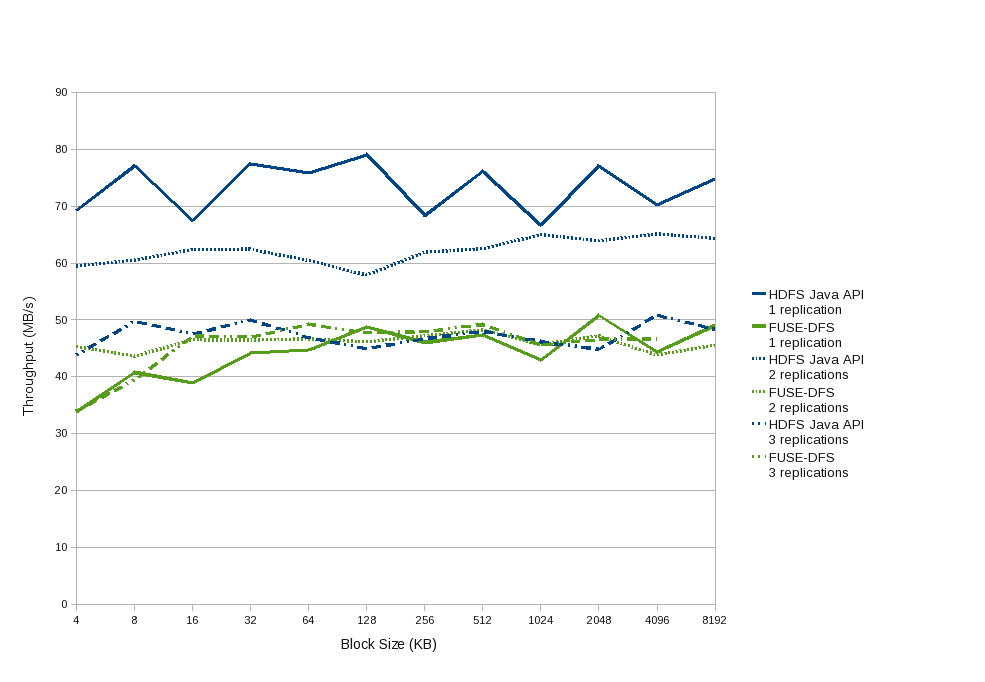
\includegraphics[totalheight=.25\textheight,
width=.75\textwidth,bb=0 0 985 682, scale=0.50]{images/WriteThroughput-4Datanodes-Line.png}
 % WriteThroughput-4Datanodes-Line.png: 985x682 pixel, 72dpi, 34.75x24.06 cm, bb=0 0 985 682
 \caption{\emph{FUSE-dfs versus the HDFS Java API \textit{write} throughput per block size 
for writing 15.7GB using \textit{1 Namenode} and \textit{4 Datanodes}. HDFS replication factors range from 1 to 3.}}
\end{figure}

\begin{figure}
 \centering
 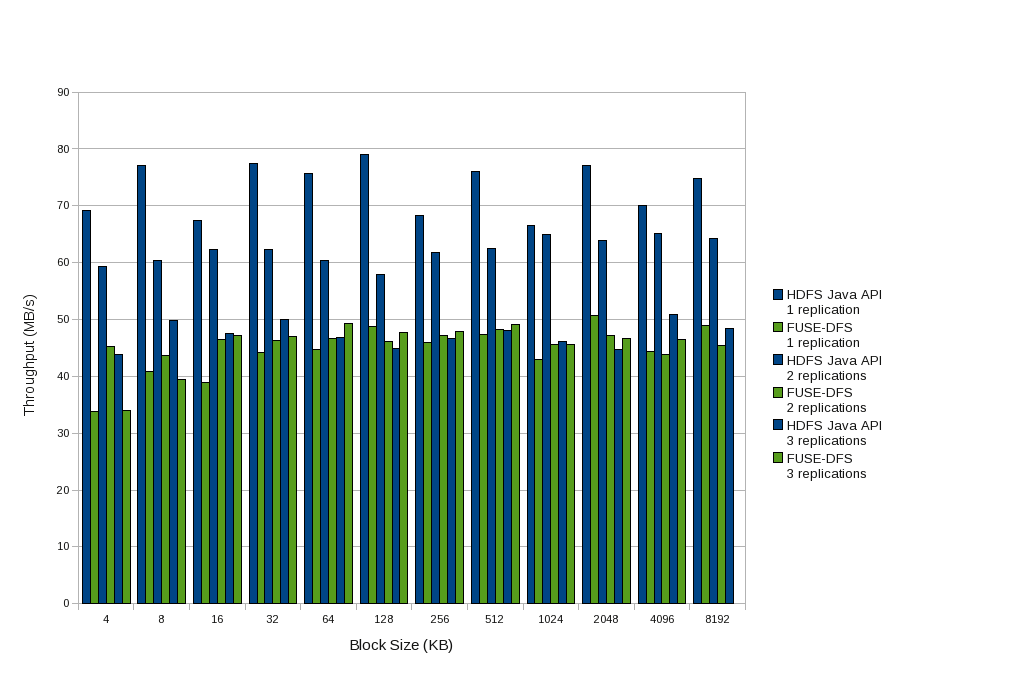
\includegraphics[totalheight=.25\textheight,
width=.75\textwidth,bb=0 0 985 682, scale=0.50]{images/WriteThroughput-4Datanodes-Bar.png}
 % WriteThroughput-4Datanodes-Line.png: 985x682 pixel, 72dpi, 34.75x24.06 cm, bb=0 0 985 682
 \caption{\emph{FUSE-dfs versus the HDFS Java API \textit{write} throughput per block size 
for writing 15.7GB using \textit{1 Namenode} and \textit{4 Datanodes}. HDFS replication factors range from 1 to 3.}}
\end{figure}

\begin{figure}
 \centering
 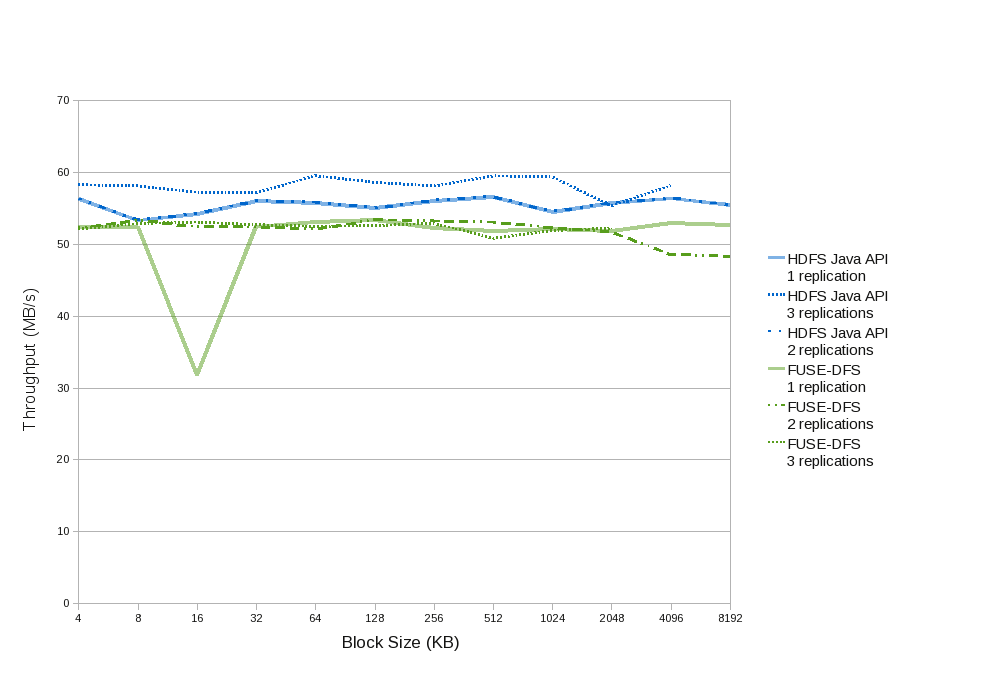
\includegraphics[totalheight=.25\textheight,
width=.75\textwidth,bb=0 0 985 682, scale=0.50]{images/ReadThroughput-4Datanodes-Line.png}
 % WriteThroughput-4Datanodes-Line.png: 985x682 pixel, 72dpi, 34.75x24.06 cm, bb=0 0 985 682
 \caption{\emph{FUSE-dfs versus the HDFS Java API \textit{read} throughput per block size 
for reading 15.7GB using \textit{1 Namenode} and \textit{4 Datanodes}. HDFS replication factors range from 1 to 3.}}
\end{figure}

\begin{figure}
 \centering
 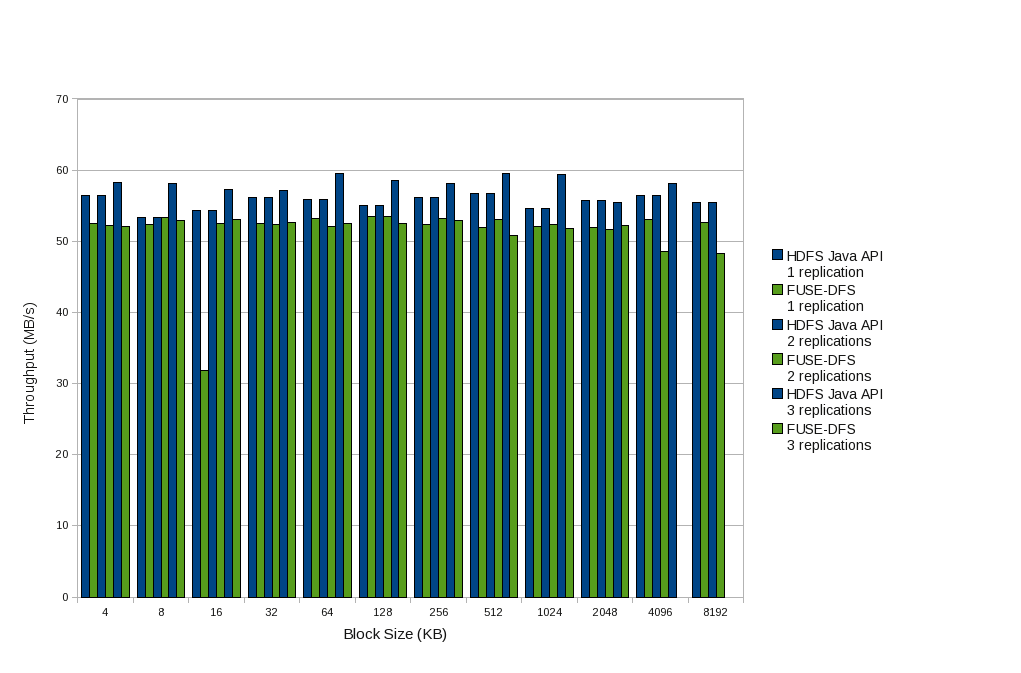
\includegraphics[totalheight=.25\textheight,
width=.75\textwidth,bb=0 0 985 682, scale=0.50]{images/ReadThroughput-4Datanodes-Bar.png}
 % WriteThroughput-4Datanodes-Line.png: 985x682 pixel, 72dpi, 34.75x24.06 cm, bb=0 0 985 682
 \caption{\emph{FUSE-dfs versus the HDFS Java API \textit{read} throughput per block size 
for reading 15.7GB using \textit{1 Namenode} and \textit{4 Datanodes}. HDFS replication factors range from 1 to 3.}}
\end{figure}

\begin{figure}
 \centering
 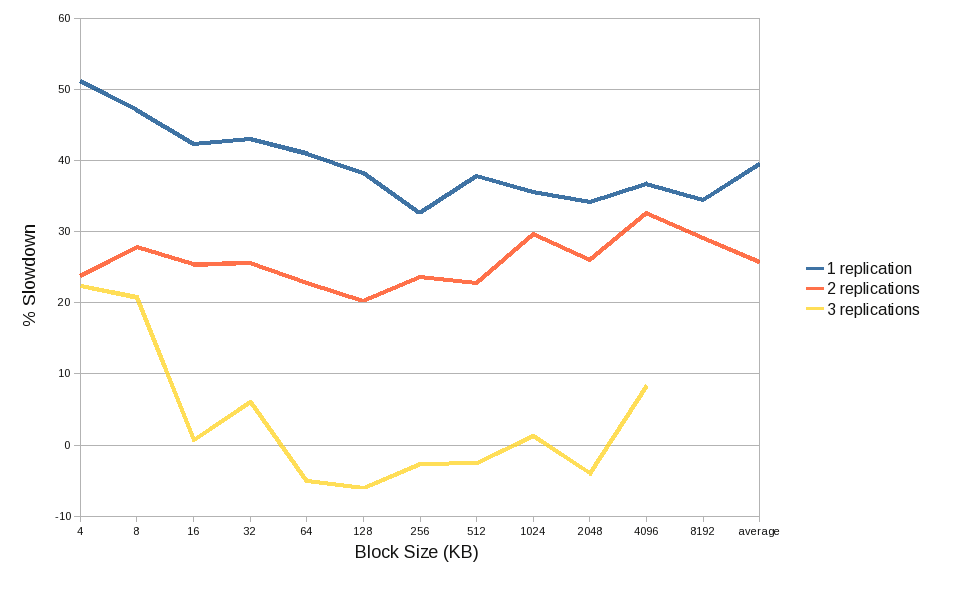
\includegraphics[totalheight=.25\textheight,
width=.75\textwidth,bb=0 0 985 682, scale=0.50]{images/WriteSlowdown-4Datanodes.png}
 % WriteThroughput-4Datanodes-Line.png: 985x682 pixel, 72dpi, 34.75x24.06 cm, bb=0 0 985 682
 \caption{\emph{Slowdown percentage of \textit{write} throughput per block size of FUSE-dfs versus the HDFS Java API}}
\end{figure}

\begin{figure}
 \centering
 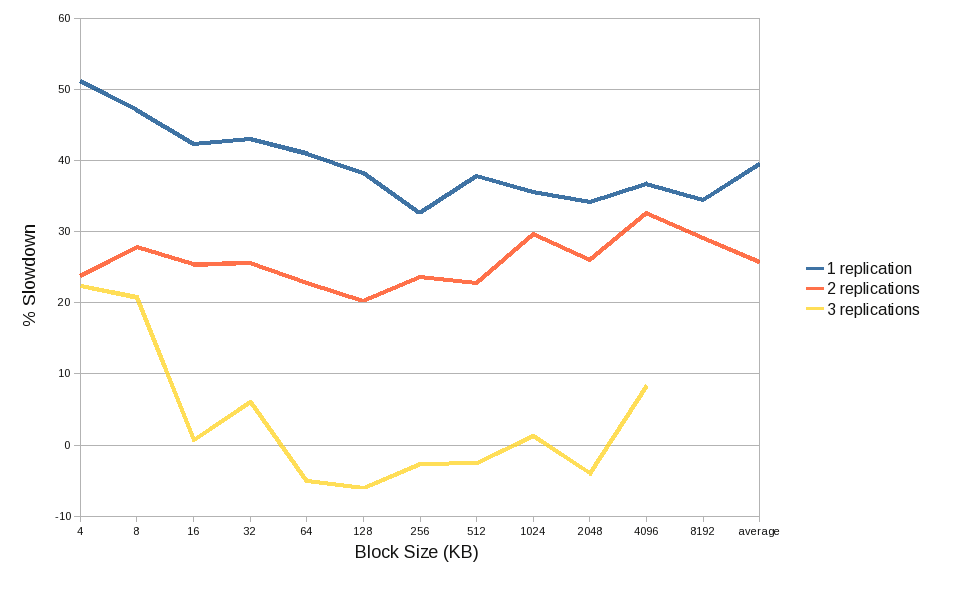
\includegraphics[totalheight=.25\textheight,
width=.75\textwidth,bb=0 0 985 682, scale=0.50]{images/WriteSlowdown-4Datanodes.png}
 % WriteThroughput-4Datanodes-Line.png: 985x682 pixel, 72dpi, 34.75x24.06 cm, bb=0 0 985 682
 \caption{\emph{Slowdown percentage of \textit{read} throughput per block size of FUSE-dfs versus the HDFS Java API}}
\end{figure}

\section{Conclusion}

\section{References}

\end{document}
